%% \section{Context effects and non-indexability}

%% \note{No index theorem; via context inversion counter-example}

The Gittins index theorem \citep{Gittins:1979} is a famous structural
result for bandit problems.  It states that in bandit problems with
independent reward distribution for each arm and geometric discounting,
the optimal policy is an \term{index policy}:  each arm is assigned a
real-valued index based on its state only, such that it is optimal to
sample the arm with greatest index.

The analogous result does \emph{not} hold for metalevel decision problems,
even when the action's values are independent (this formalized later in \dfnref{dfn:independent-actions}):

\begin{example}[Non-indexability]
Consider a metalevel probability model with three actions. 
	$U_1$ is equally likely to be $-1.5$ or $1.5$ (low mean, high variance),
	$U_2$ is equally likely to be $0.25$ or $1.75$ (high mean, low variance),
	and $U_3=\lambda$ has a known value (the context).
The two computations are to observe exactly $U_1$ and $U_2$, respectively, each with cost $0.2$.
The corresponding metalevel MDP has 9 states and can be solved exactly.
\figref{fig:swap-counterex} plots $Q^*_\lambda(s_0,U_i) - Q^*_\lambda(s_0,\bot)$ as a function of the known value $\lambda$.
As the context $\lambda$ varies the optimal action inverts from observing 1 to observing 2.
Inversions like this are impossible for index policies.
\end{example}

\begin{figure}[htb]
\centering
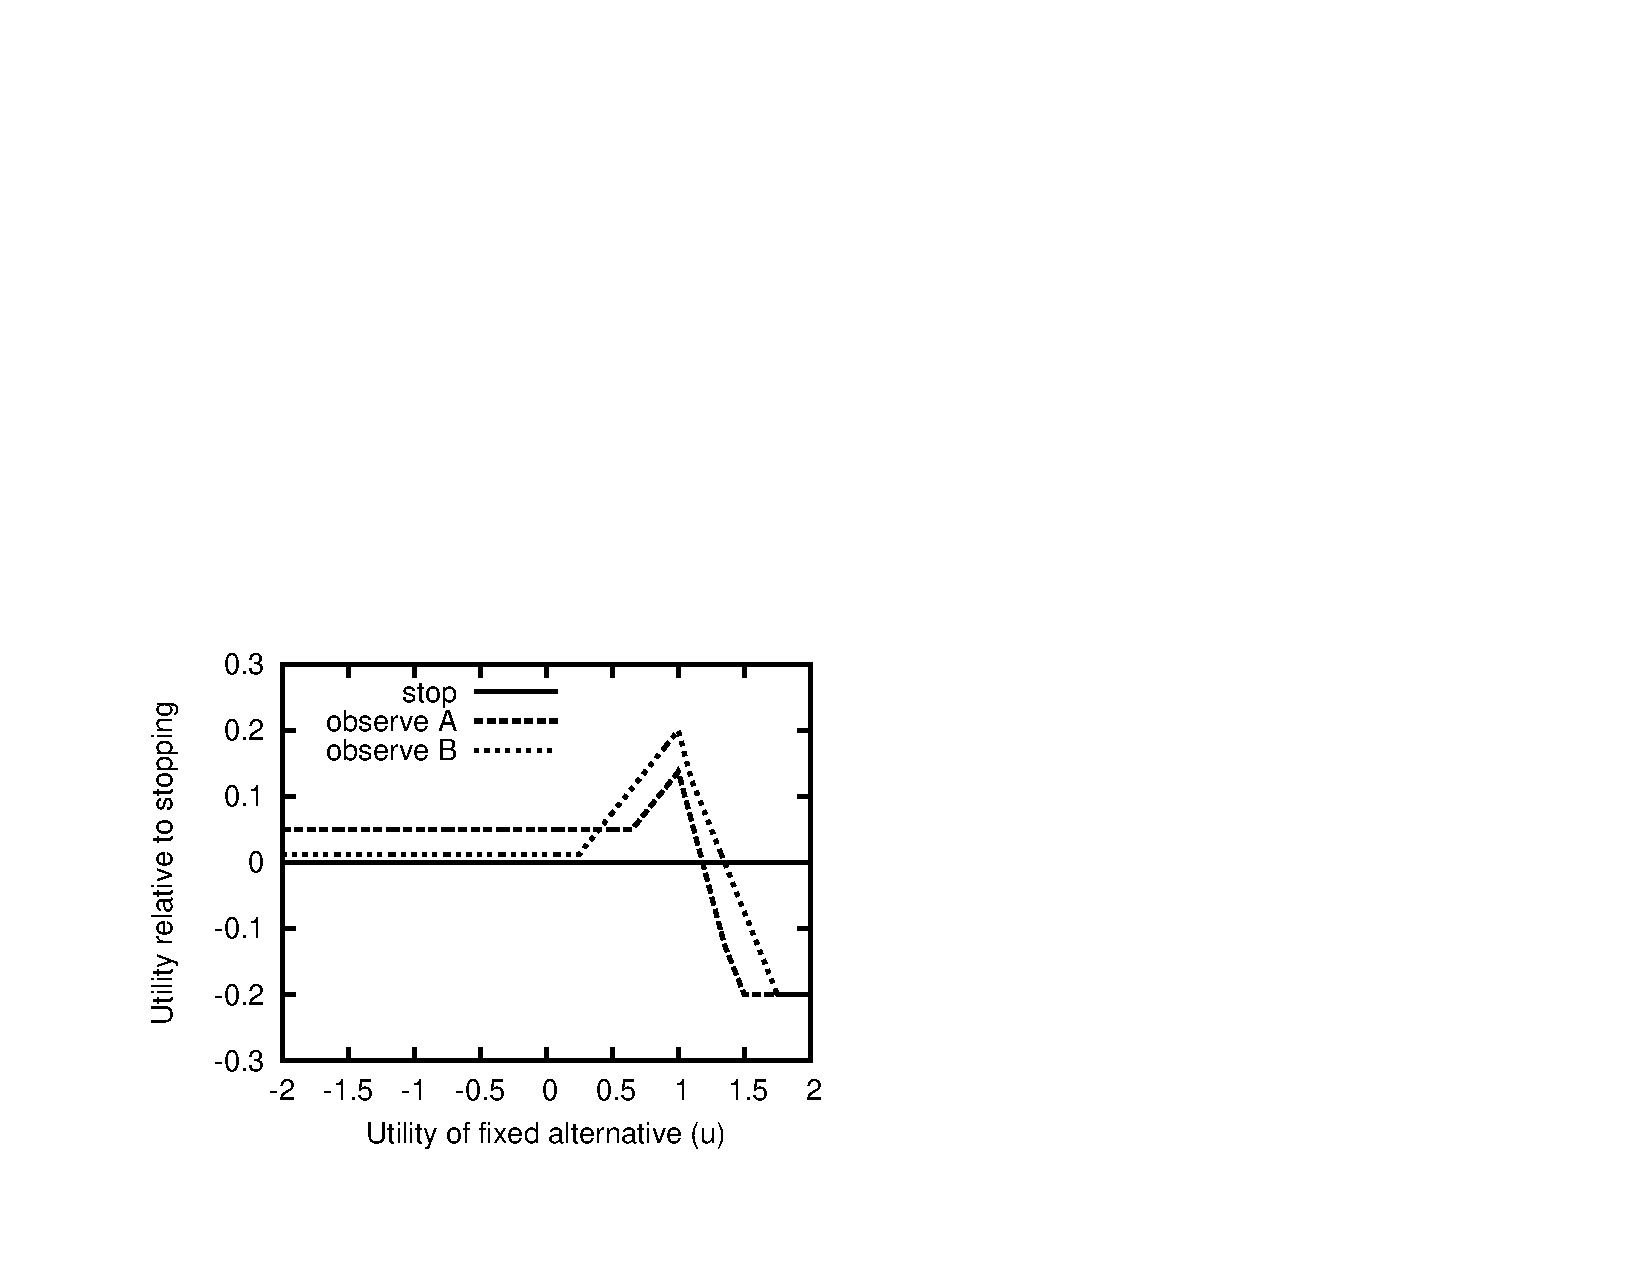
\includegraphics[scale=0.7, trim=90 70 400 300]{swap-counterex.pdf}
\caption{Optimal Q-values of computing relative to stopping as a function of the utility of the fixed alternative.  Note the inversion
where for low $\lambda$ observing action~$1$ is strictly optimal, while for medium $\lambda$ observing action~$2$ is strictly optimal.}
\label{fig:swap-counterex}
\end{figure}

\begin{comment}
	set samples 1000

	max(x,y) = x>y ? x : y
	max3(x,y,z) = max(max(x,y),z)

	q0(u) = max(1,u)
	qa(u) = 0.5*max3(u, 1.5, -0.2 + 0.5*max(u,1.5) + 0.5*max(u, 1.75)) + 0.5*max3(u, 1, -0.2 + 0.5*max(u,0.25) + 0.5*max(u, 1.75)) - 0.2
	qb(u) = 0.5*max3(u, 0.25, -0.2 + 0.5*max(u,1.5) + 0.5*max(u, 0.25)) + 0.5*max3(u, 1.75, -0.2 + 0.5*max(u,1.75) + 0.5*max(u, 1.75)) - 0.2

	set terminal postscript enhanced linewidth 2
	set size 0.5,0.5
	set output "swap-counterex.ps"
	set xlabel "Utility of fixed alternative ({/Symbol l})"
	set ylabel "Utility relative to stopping"
	set xtics 0.5
	set ytics 0.1
	set key left top
	plot [u=-2:2] [-0.3:0.3] 0 title "stop" with lines lw 2, qa(u)-q0(u) title "observe 1" with lines lw 2, qb(u)-q0(u) title "observe 2" with lines lw 2	
\end{comment}




%% \note{Theorem: /stopping/ context effect occurs only for a single convex interval of
%%    context value (how general can we make this?)}

There is, however, a restriction on what kind of influence the context can have:

\begin{dfn}\label{dfn:context}
	Given a metalevel decision problem $M=(S,s_0,A_s,T,R)$, and a constant $\lambda\in\R$,
	define $M_\lambda = (S,s_0,A_s,T,R_\lambda)$ to be $M$ with an additional action of known 
	value $\lambda$, defined by:
	\begin{align*}
		R_\lambda(s,E,s')      &= R(s,E,s') \\
		R_\lambda(s,\bot,\bot) &= \max\{\lambda, R(s,\bot,\bot)\}
	\end{align*}
\end{dfn}

Note this is equivalent to adding an extra arm with constant value $U_{k+1}=\lambda$.

\begin{thm}
	Given a metalevel decision problem $M=(S,s_0,A_s,T,R)$, 
	there exists a real interval $I(s)$ for every state $s\in S$ such that
	it is optimal to stop in state $s$ in $M_\mu$ iff $\mu\notin I(s)$.
	Furthermore, $I(s)$ contains $\max_i\mu_i(s)$ whenever it is nonempty.
\end{thm}

\begin{hiddenproof}
	\begin{proof}
	With $m(s) = \max_i\mu_i(s)$, the utility of a policy $\pi$ starting in state $s$ of $M_\mu$ is
	\[
		V^\pi_{M_\mu}(s) = \IE_{\pi}[-c\,N + \max(\mu,m(S_N)) \given S_0=s]
	\]
	and the utility of stopping in this state $\max(\mu,m(s_0))$.
	We wish to show that the set of $\mu$ such that
	\[
		\max_\pi \IE_{\pi}[-c\,N + \max(\mu,m(S_N)) - \max(\mu,m(S_0)) \given S_0=s] \le 0
	\]
	forms an interval.  

	Observe that for any random variable $X$, 
		$\IE[\max(\mu,X)]$ is monotonically increasing in $\mu$ with subderivative between zero and one.
	As a result, for any $v_1$
		$\IE[\max(\mu,X)] - \max(\mu,v_1)$ 
		is monotonically increasing for $\mu<v$, 
		and monotonically decreasing thereafter.
	Therefore, the set if $\mu$ such that this expression is at most $v_2$ forms an interval, containing $v_1$ if non-empty.

	Applying this with $v_1 = m(s_0)$ and $v_2=\IE_{\pi}[c\,N]$, and observing that the union of intervals containing
	a point is an interval containing that point, gives the result.
	\end{proof}	
\end{hiddenproof}

%% \note{Example showing that choice between computations to perform 
%% can vary arbitrarily many times?  Does one exist?}